% SpaceX IPO -- Teaching Deck
% Companion to "SpaceX: To the Moon, or Back to Earth?"
% Compile with:  xelatex SpaceX_IPO_Slides.tex   (run twice)
% Requires beamer + metropolis (MiKTeX auto-installs on first run).

\documentclass[aspectratio=169,11pt]{beamer}

% Self-contained clean theme (no external metropolis dependency).
\usetheme{default}
\usecolortheme{default}

\usepackage{booktabs}
\usepackage{graphicx}
\usepackage{appendixnumberbeamer}

% --- Palette ---
\definecolor{accent}{HTML}{1F3A5F}
\definecolor{accentred}{HTML}{B23A48}
\definecolor{softgray}{HTML}{4A4A4A}

% --- Strip default chrome ---
\setbeamertemplate{navigation symbols}{}
\setbeamercolor{structure}{fg=accent}
\setbeamercolor{frametitle}{fg=accent}
\setbeamercolor{title}{fg=accent}
\setbeamercolor{alerted text}{fg=accentred}
\setbeamercolor{section in toc}{fg=accent}
\setbeamerfont{frametitle}{series=\bfseries,size=\large}
\setbeamerfont{title}{series=\bfseries,size=\LARGE}
\setbeamertemplate{itemize item}{\color{accent}\textbullet}
\setbeamertemplate{itemize subitem}{\color{accent}\textendash}
\setbeamersize{text margin left=10mm, text margin right=10mm}

% Frametitle with an accent rule under it
\setbeamertemplate{frametitle}{%
  \nointerlineskip
  \vspace{2mm}\hspace{1mm}%
  {\usebeamerfont{frametitle}\usebeamercolor[fg]{frametitle}\insertframetitle}\par
  \vspace{1mm}%
  {\color{accent}\rule{\dimexpr\paperwidth-6mm\relax}{0.6pt}}%
  \vspace{1mm}%
}

% Footer: short title left, page x/N right
\setbeamertemplate{footline}{%
  \leavevmode%
  \hbox{\hspace{4mm}\color{softgray}\footnotesize\insertshorttitle\hfill
        \color{softgray}\footnotesize\insertframenumber\,/\,\inserttotalframenumber\hspace{4mm}}%
  \vspace{2mm}%
}

\setbeamertemplate{section page}{%
  \begin{centering}
    \vfill
    {\usebeamerfont{title}\usebeamercolor[fg]{title}\insertsectionhead}\par
    \vspace{2mm}{\color{accent}\rule{0.3\paperwidth}{0.6pt}}
    \vfill
  \end{centering}%
}
\AtBeginSection[]{\frame{\sectionpage}}

\title[SpaceX: Flip or Hold?]{SpaceX: To the Moon, or Back to Earth?}
\subtitle{A Retail Investor's Flip-or-Hold Decision}
\author{Teaching Deck}
\institute{HBS-style case \textbar{} Event date: June 19, 2026}
\date{}

\begin{document}

\maketitle

% ============================================================
\begin{frame}{The decision at hand}
  \begin{itemize}
    \item \textbf{Protagonist:} Maya Chen, individual (retail) investor
    \item \textbf{Position:} 50 SPCX shares allocated at the \$135 IPO price (\$6,750)
    \item \textbf{Date:} Friday, June 19, 2026 --- end of the first week of trading
    \item \textbf{Current price:} \$185.00 \quad (\textbf{+37\%} in one week; peaked at \$225.64 on Mon Jun 15)
    \item \textbf{The choice:} \alert{sell now and lock in the gain, or hold?}
  \end{itemize}
\end{frame}

% ============================================================
\section{The company}

\begin{frame}{SpaceX, in one slide}
  \begin{columns}[T,onlytextwidth]
    \column{0.5\textwidth}
      \textbf{Two pillars:}
      \begin{itemize}
        \item \textbf{Launch \& transport:} Falcon 9, Falcon Heavy, Starship (in dev)
        \item \textbf{Starlink:} satellite internet, ~10M subs / ~160 countries
      \end{itemize}
    \column{0.45\textwidth}
      \textbf{Founded 2002 by Elon Musk.}
      \begin{itemize}
        \item Dominant orbital launch provider
        \item Private until the 2026 IPO
        \item Musk retains commanding voting control
      \end{itemize}
  \end{columns}
\end{frame}

% ============================================================
\section{The offering}

\begin{frame}{The largest IPO in history}
  \begin{itemize}
    \item \textbf{Offer price:} \$135 / share
    \item \textbf{Shares:} 555.6M \quad \textbf{Raised:} ~\$75B (record)
    \item \textbf{Valuation at offer:} ~\$1.75T
    \item \textbf{Listing:} Nasdaq: SPCX \quad \textbf{Priced:} Jun 11, 2026
  \end{itemize}

  \vspace{0.5em}
  \alert{Unusual feature:} ~30\% of the deal allocated to retail (~3x typical), via Robinhood, Fidelity, E*TRADE, Schwab, SoFi.
\end{frame}

\begin{frame}{Exhibit: retail allocation, SPCX vs typical IPO}
  \begin{center}
    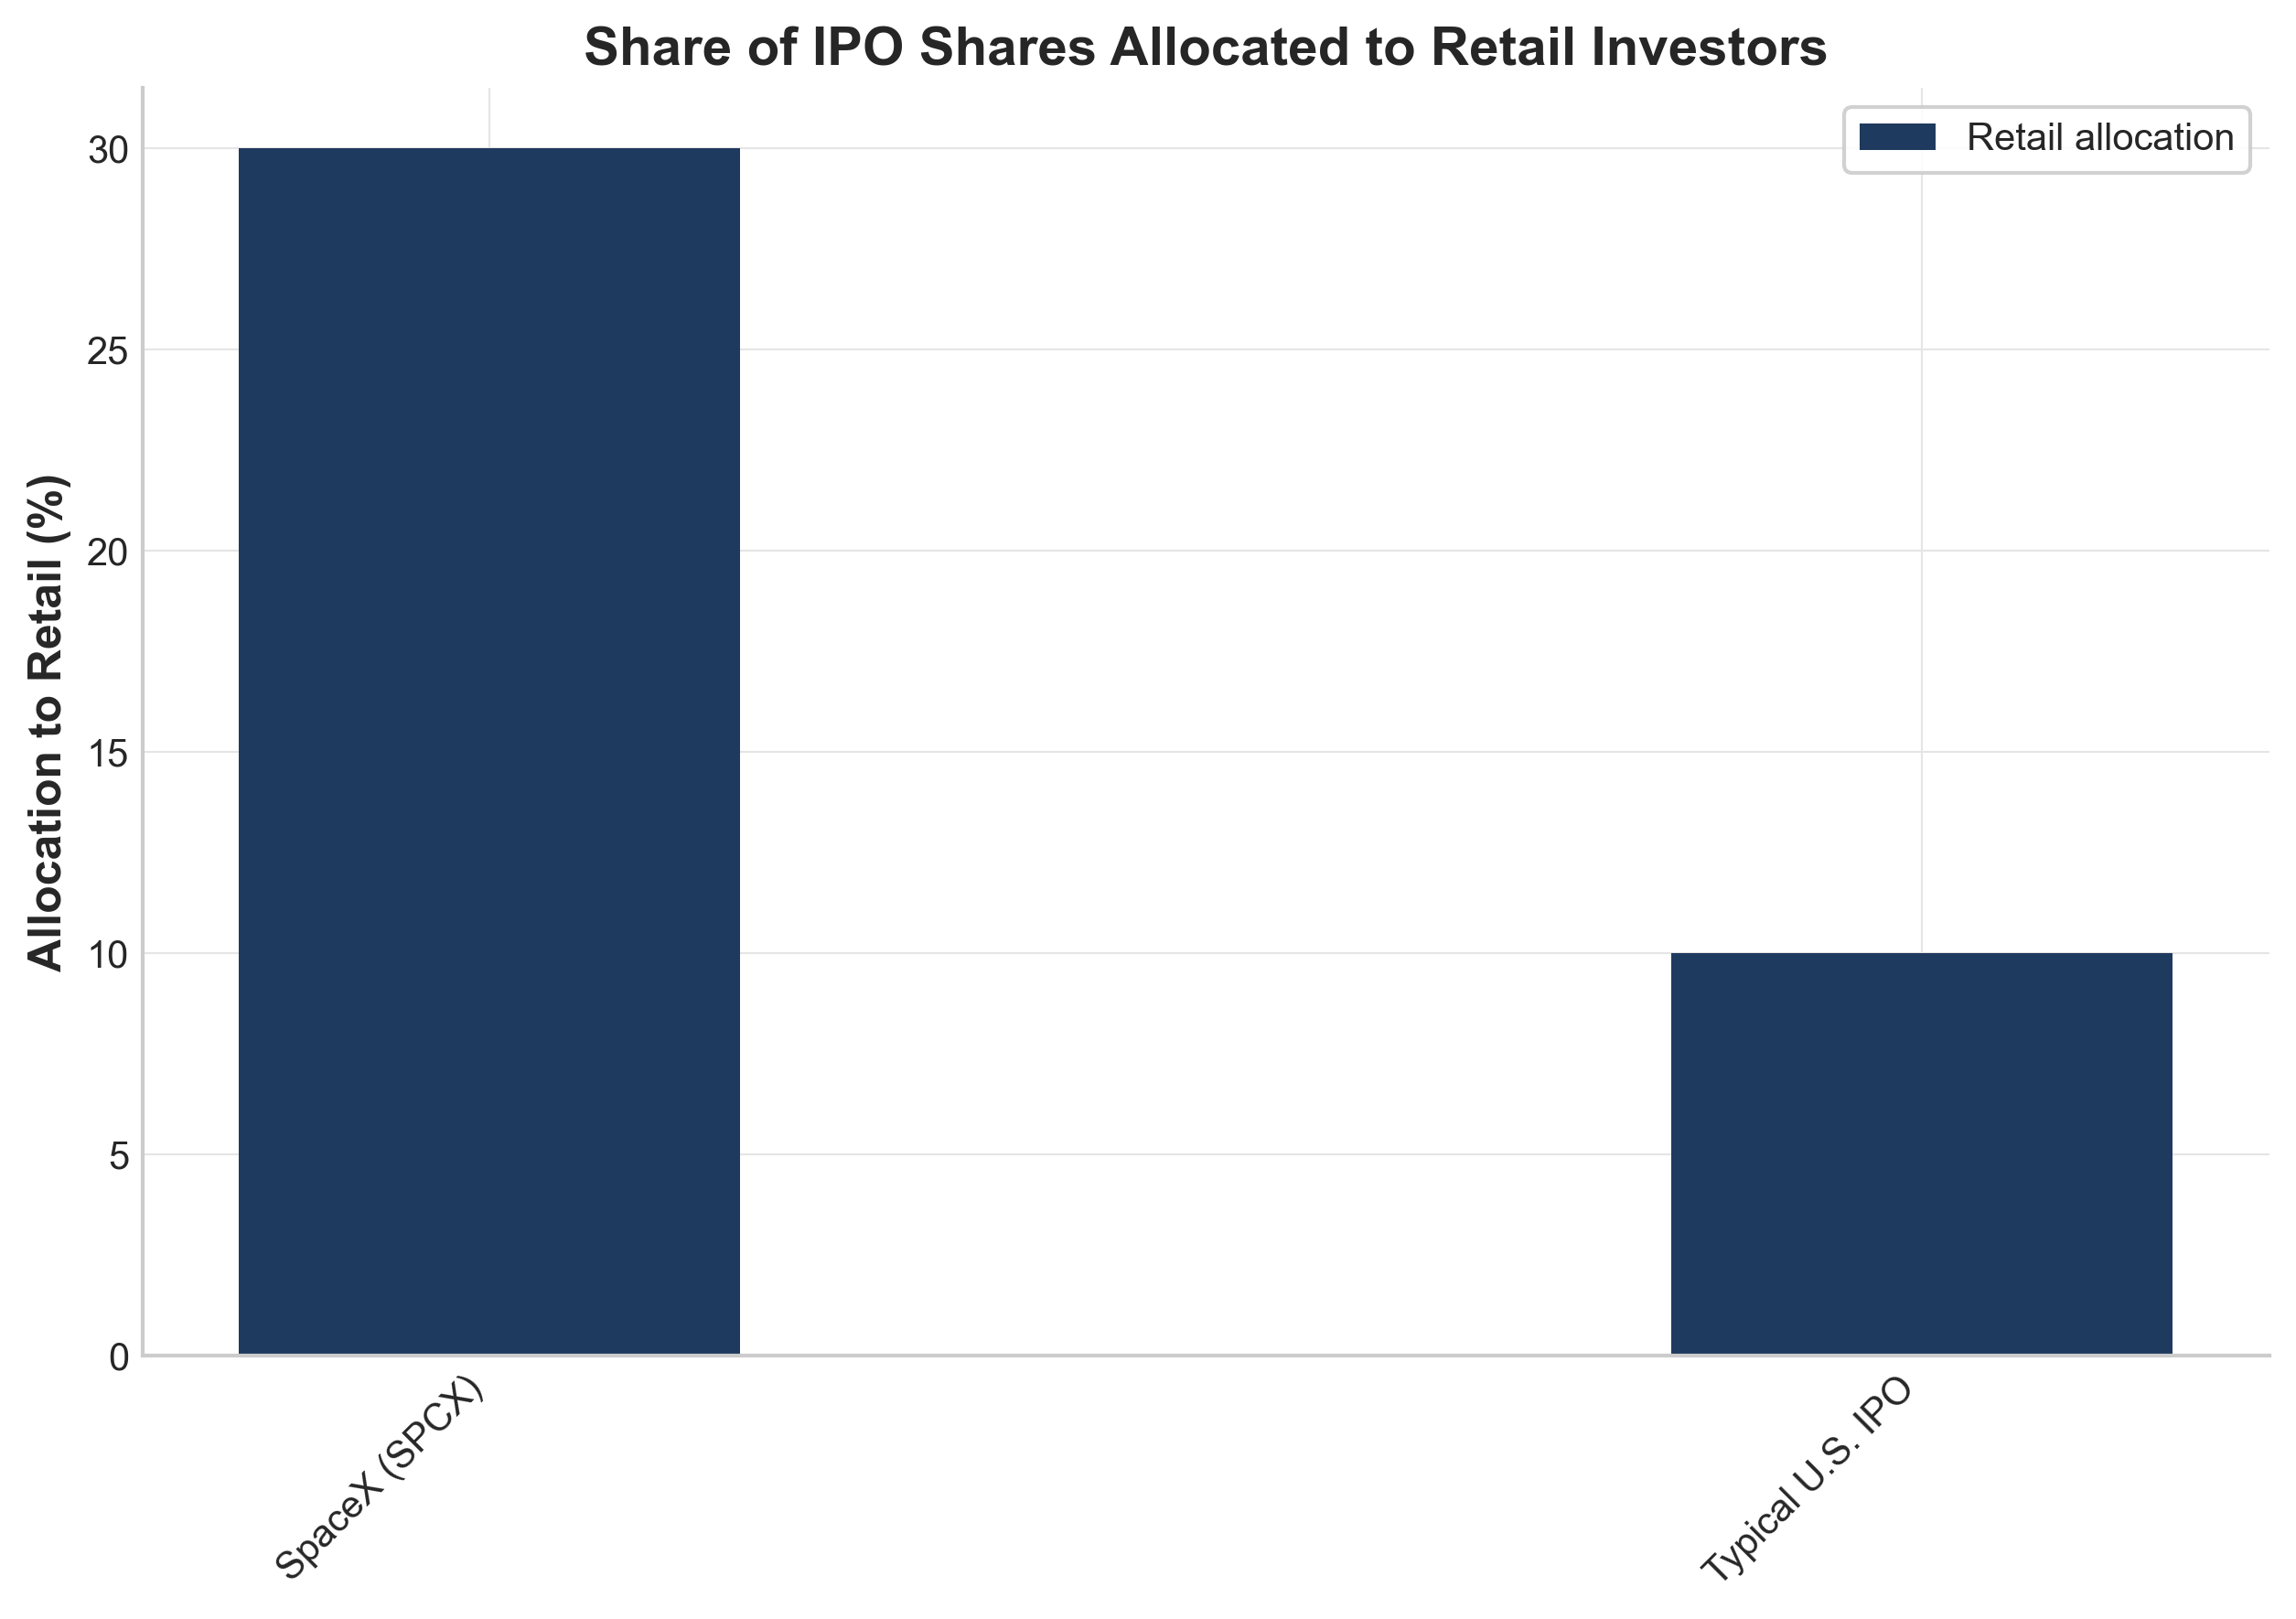
\includegraphics[height=0.65\textheight]{figures/exhibit_retail_allocation.png}
  \end{center}
  \tiny \textbf{Source:} Reuters (Mar 2026); CNBC (May 2026); Robinhood IPO Access.
\end{frame}

% ============================================================
\section{The first week}

\begin{frame}{Exhibit: SPCX first-week price action}
  \begin{center}
    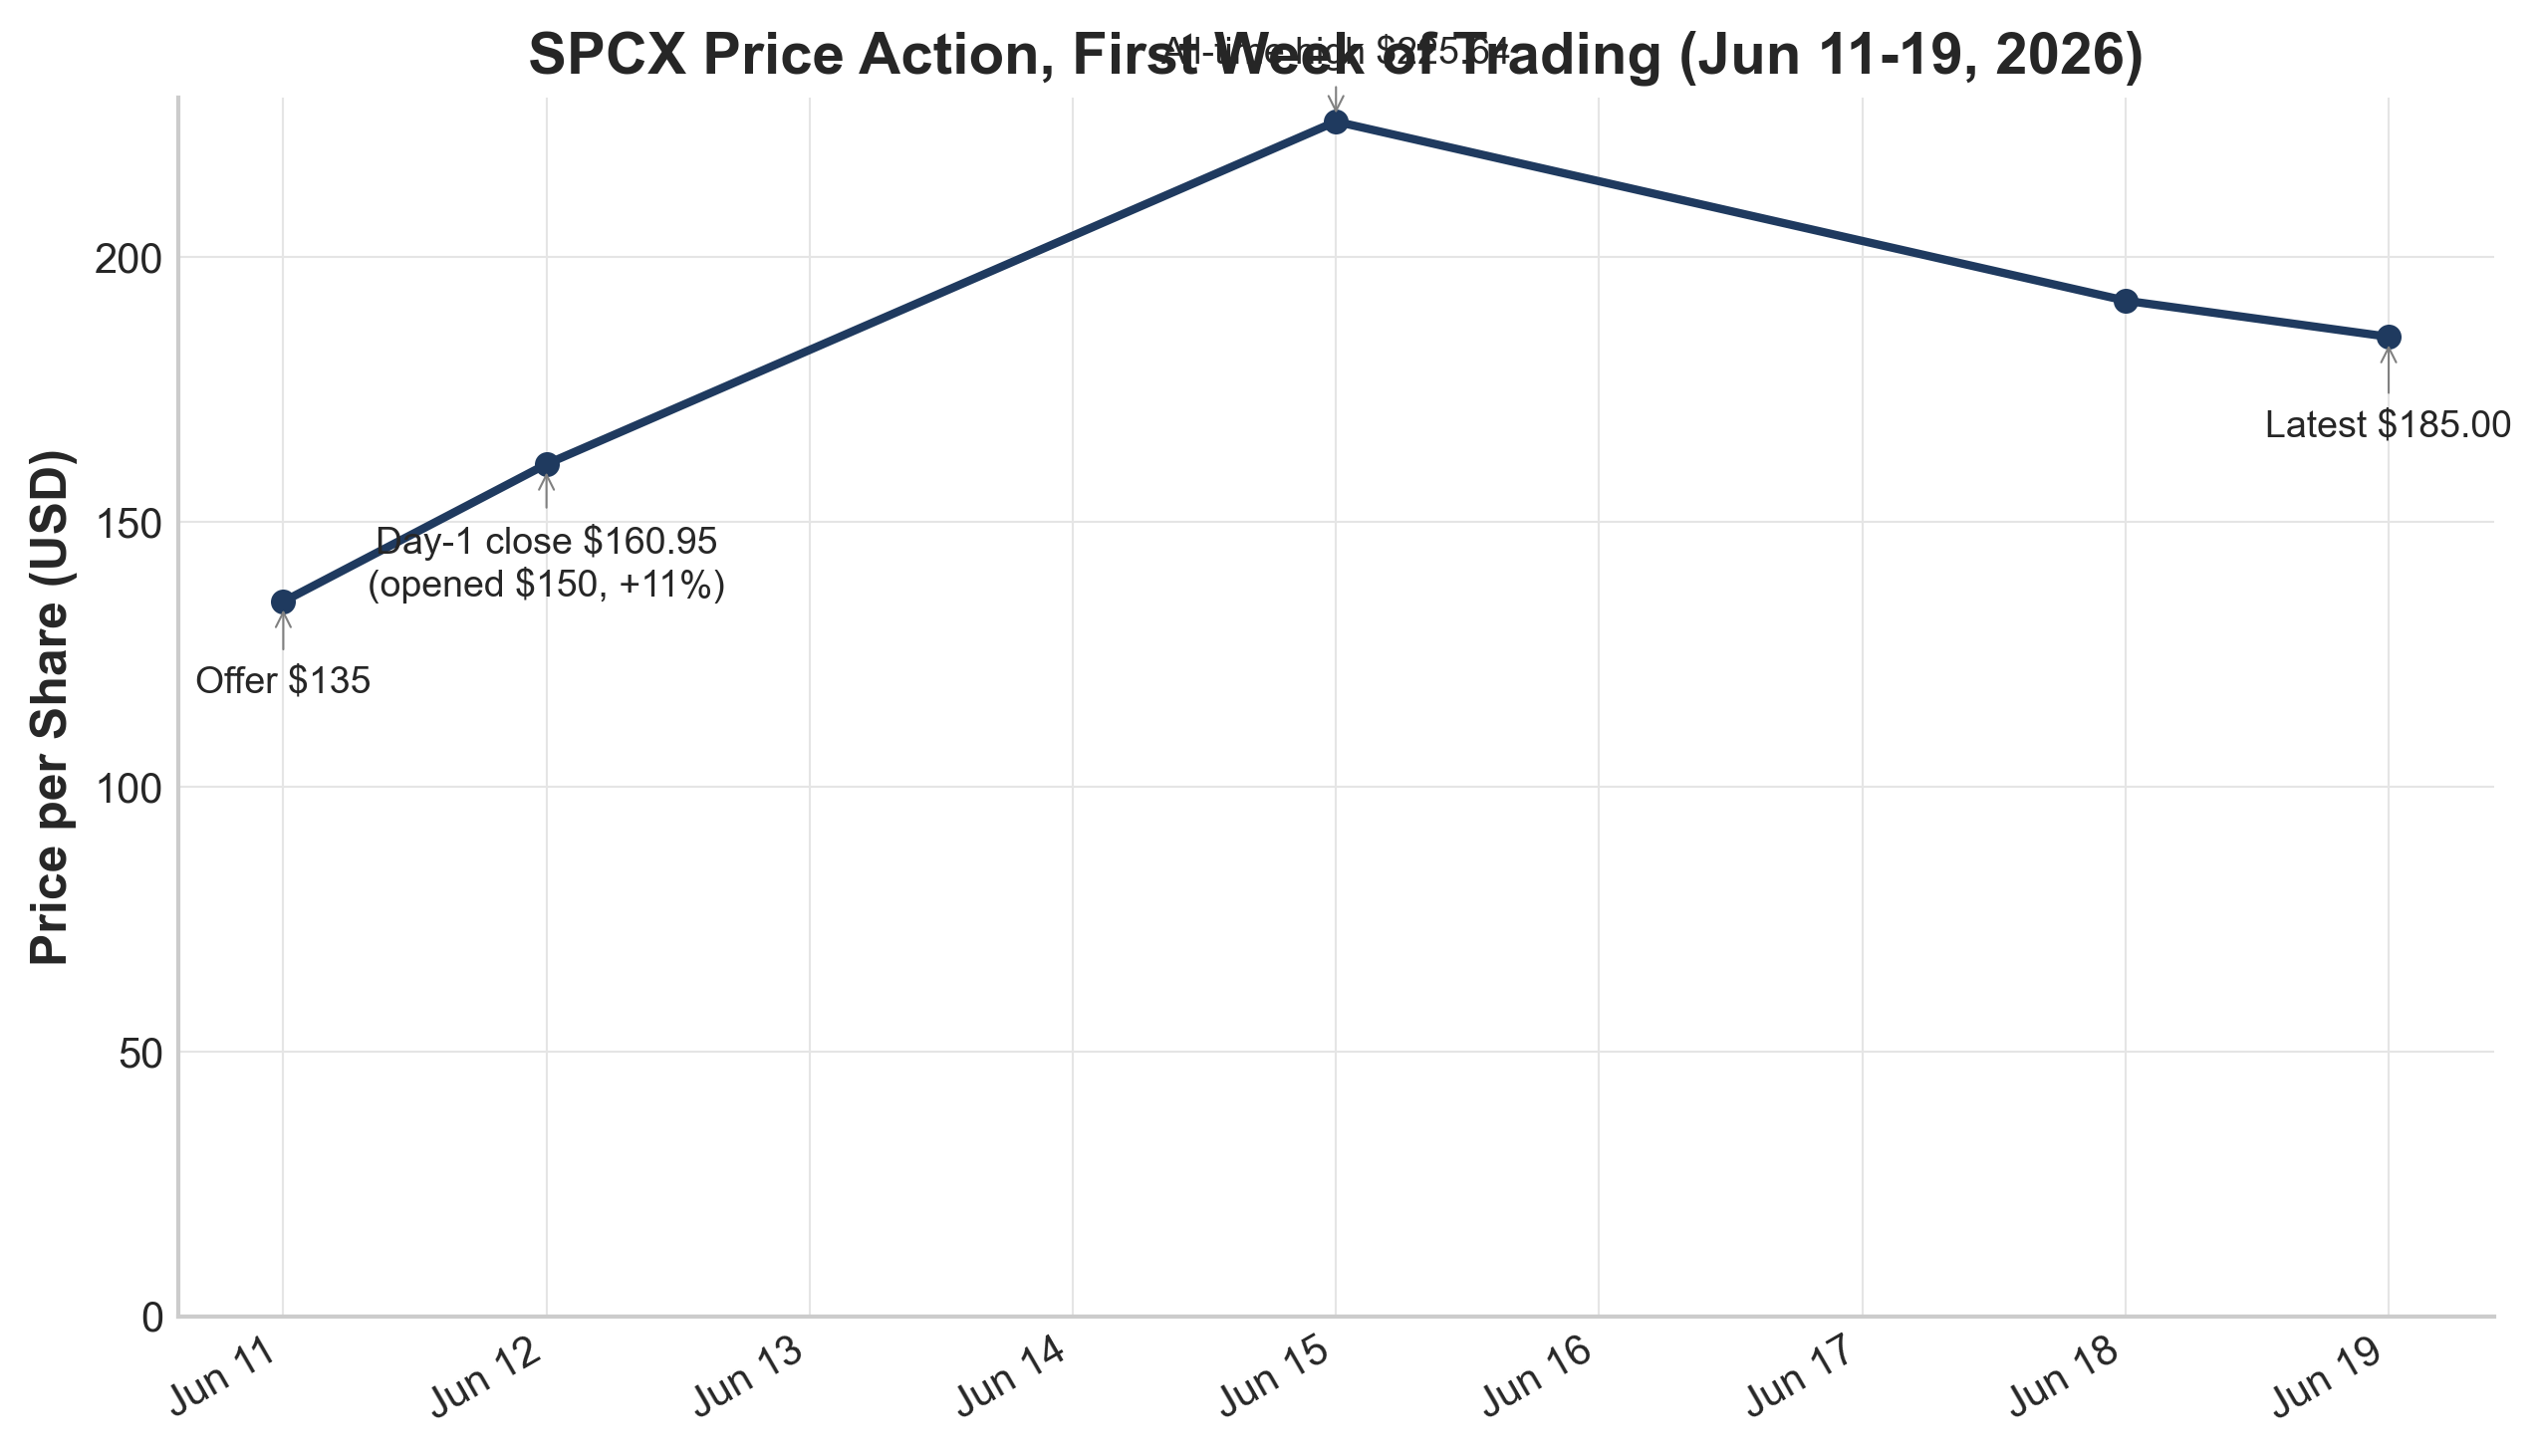
\includegraphics[height=0.68\textheight]{figures/exhibit_price_action.png}
  \end{center}
  \tiny \textbf{Source:} Investing.com, TradingView, CBS News, NBC News, CNN Markets. Points combine offer price, selected closes, and the intraday ATH.
\end{frame}

\begin{frame}{A week of extremes}
  \begin{itemize}
    \item \textbf{Jun 12 (day 1):} opened \$150 (+11\%), closed \$160.95 (+19\%)
    \item \textbf{Jun 15 (Mon):} intraday high \$225.64 --- market cap briefly > \$2.3T
    \item \textbf{Jun 18--19:} drifted to \$191.82, then \$185.00
    \item \alert{Down ~18\% from the peak by Friday}
  \end{itemize}
  \vspace{0.3em}
  Bulls: healthy profit-taking after a hot debut.\\
  Bears: the euphoria is already fading.
\end{frame}

% ============================================================
\section{The numbers}

\begin{frame}{Exhibit: 2025 revenue mix}
  \begin{center}
    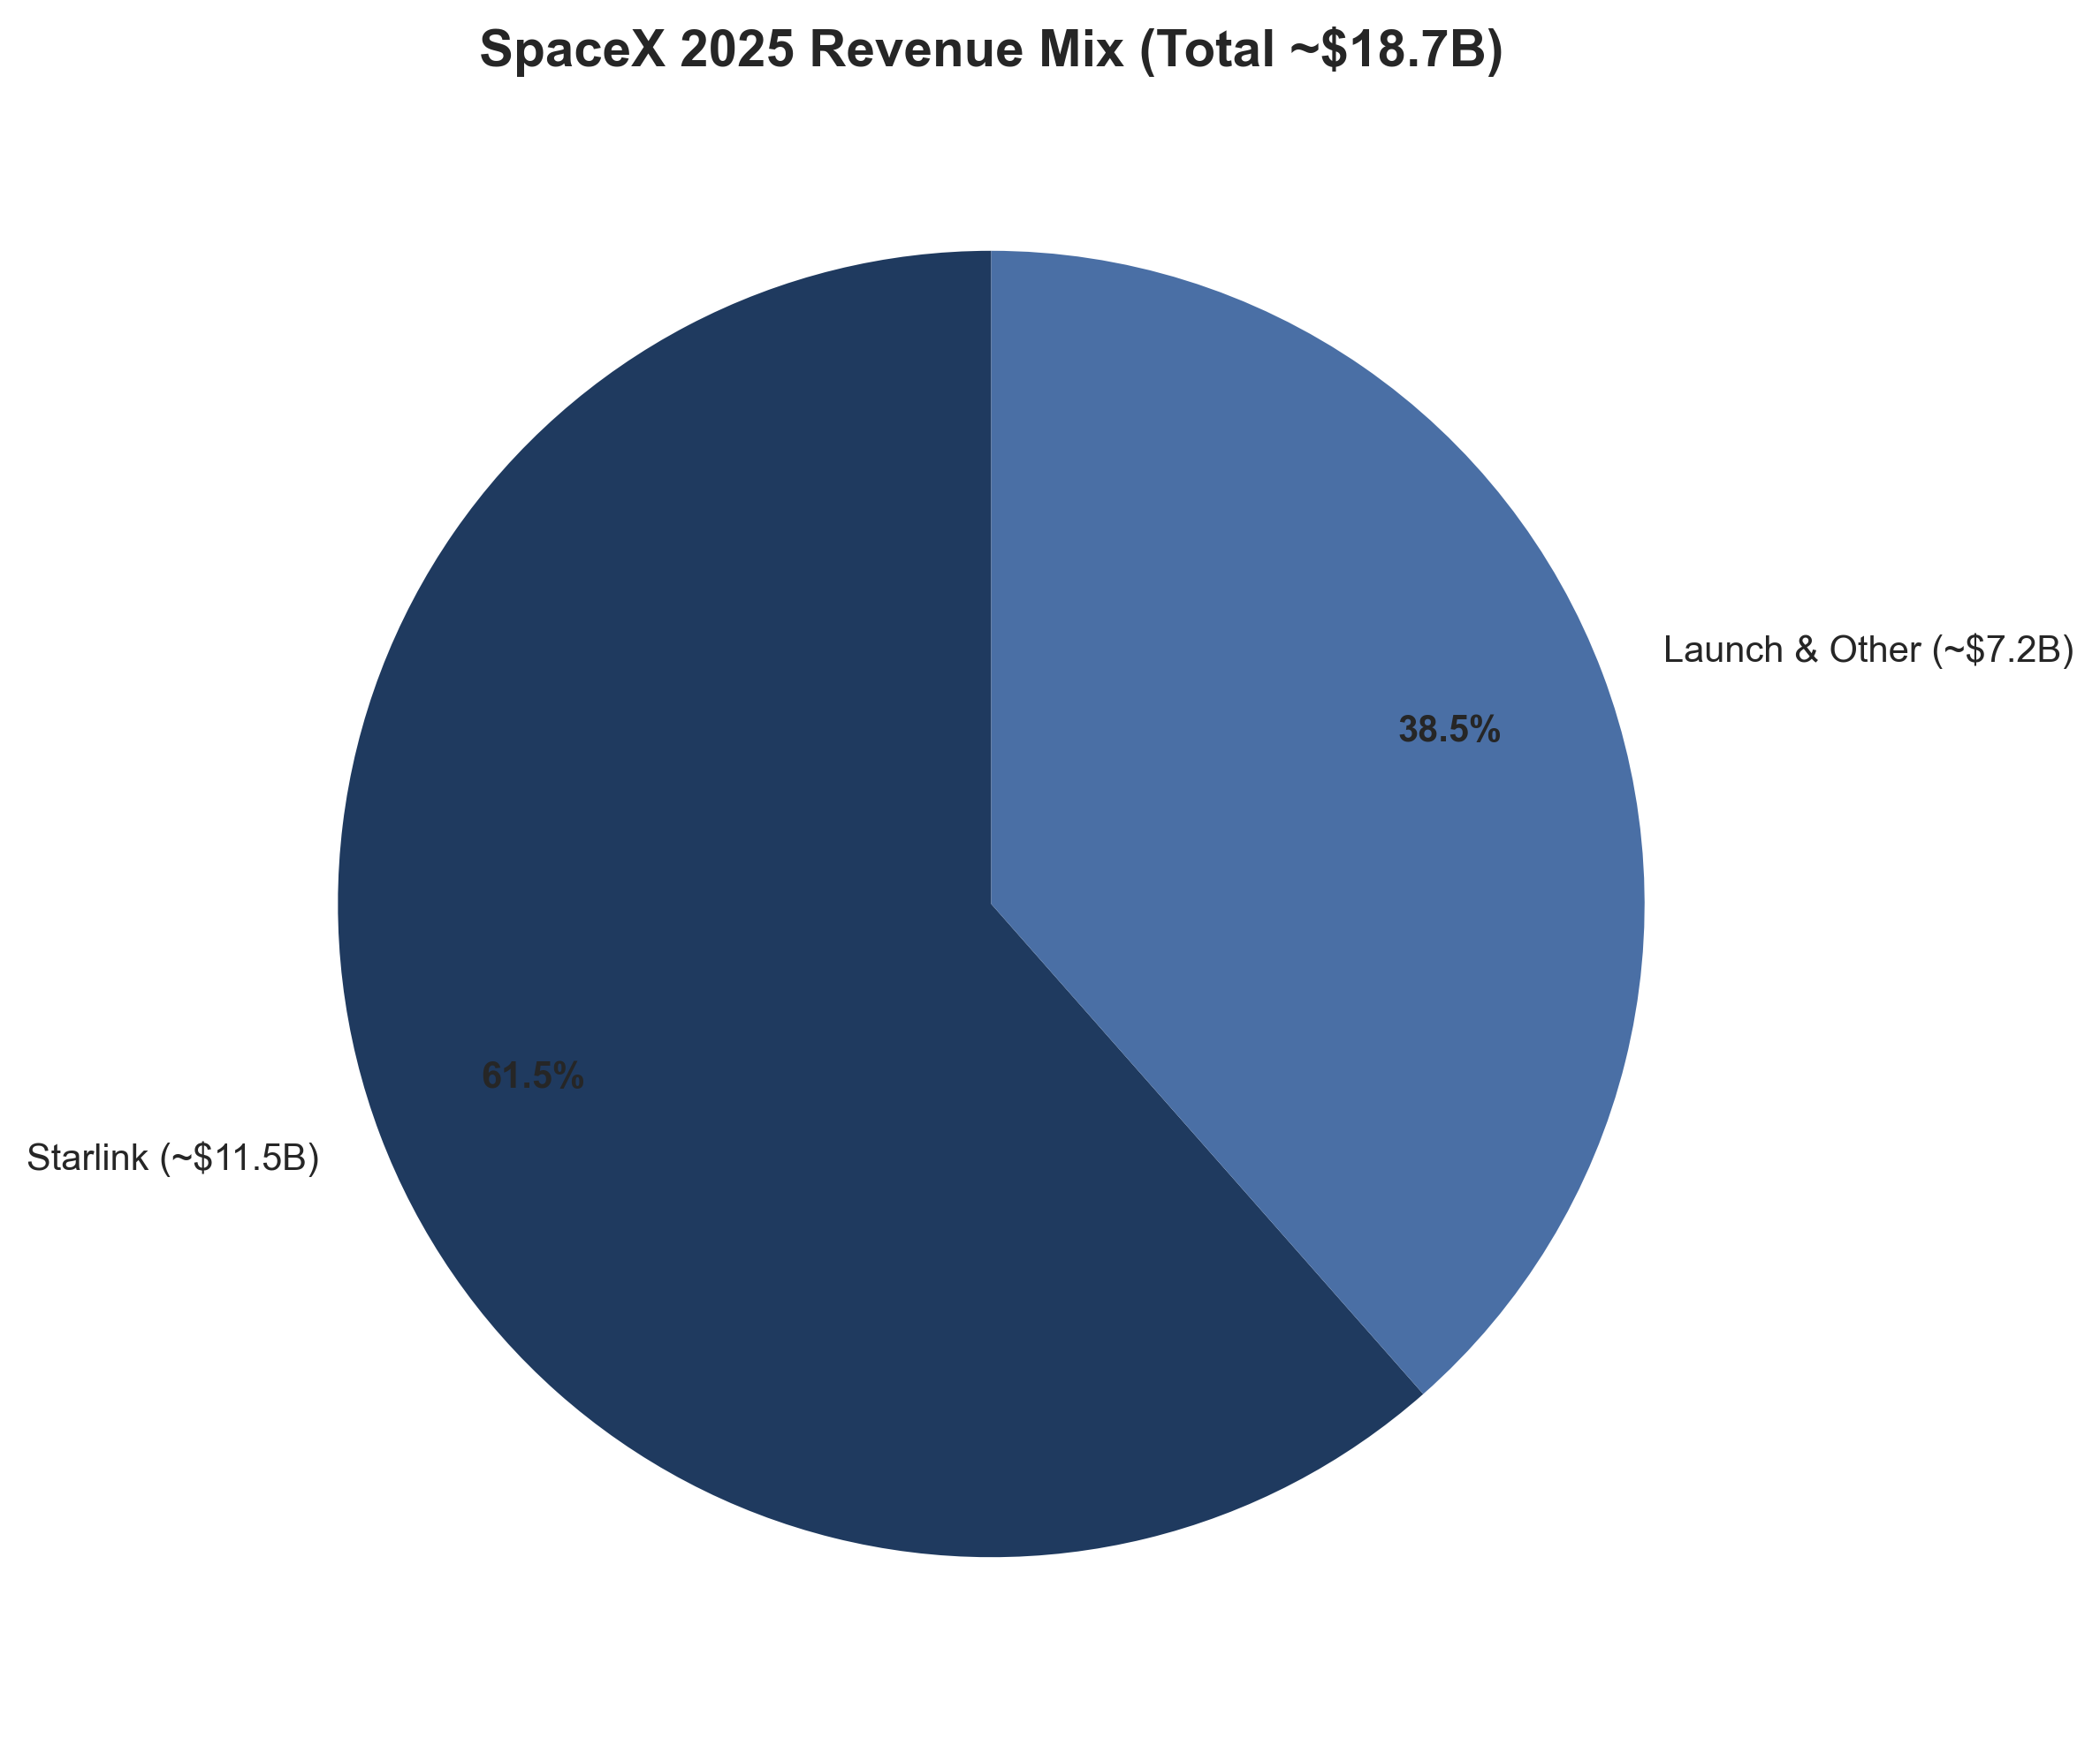
\includegraphics[height=0.62\textheight]{figures/exhibit_revenue_mix.png}
  \end{center}
  \tiny \textbf{Source:} SpaceX S-1 (SEC); Morningstar; Sacra. Starlink is the \emph{sole} profitable segment.
\end{frame}

\begin{frame}{The valuation tension}
  \begin{itemize}
    \item Consolidated 2025 revenue: ~\$18.7B (+33\% YoY)
    \item \textbf{Starlink:} ~\$11.5B, profitable, high-margin, ~60\% of revenue
    \item \textbf{Everything else} (launch, Starship, Mars): loss-making, capex-heavy
    \item Consolidated result: \alert{GAAP net loss (~\$4.9B); adj.\ EBITDA positive (~\$6.6B)}
  \end{itemize}
  \vspace{0.4em}
  At ~\$2T market cap / ~\$18.7B revenue $\Rightarrow$ \textbf{100x+ revenue multiple.}\\
  Defensible only if you believe Starlink gets very large --- and you credit Starship for free.
\end{frame}

% ============================================================
\section{Risk factors}

\begin{frame}{What the S-1 flags}
  \begin{itemize}
    \item \textbf{Key-person risk:} Musk named explicitly; runs multiple public companies
    \item \textbf{Founder control:} commanding voting power; public float has little say
    \item \textbf{Starlink dependence:} sole profitable segment funds the rest
    \item \textbf{Declining ARPU + competition} as Starlink pushes beyond rural markets
    \item \textbf{Starship:} large capex, uncertain timeline, no near-term Mars revenue
    \item \textbf{Related-party deals:} large disclosed purchases from Tesla
  \end{itemize}
\end{frame}

% ============================================================
\section{The decision}

\begin{frame}{Sell (flip)}
  \begin{itemize}
    \item +37\% in a week, before the weekend
    \item Lock in a real return; sleep through the volatility
    \item \textbf{But:} short-term capital gains tax on the profit
    \item \textbf{But:} 60-day lockout from future IPO allocations under IPO Access
    \item Miss further upside if SPCX keeps climbing
  \end{itemize}
\end{frame}

\begin{frame}{Hold}
  \begin{itemize}
    \item Starlink: fast-growing, cash-generative, wide moat
    \item Reusable launch: no real competitor
    \item Starship / Mars: free option, unbounded upside
    \item \textbf{But:} 100x+ revenue; consolidative losses
    \item \textbf{But:} key-person + governance risk; already gave back 18\% from the peak
    \item ``Many have regretted selling a Musk company early.''
  \end{itemize}
\end{frame}

\begin{frame}{}
  \vfill
  \begin{center}
    {\Huge\bfseries\color{accent} Sell or hold --- and why?}
  \end{center}
  \vfill
\end{frame}

% ============================================================
\section{Discussion}

\begin{frame}{Discussion questions}
  \begin{enumerate}
    \item Should Chen sell at \$185 or hold? What single fact would change her mind?
    \item What must be true for 100x+ revenue to be defensible?
    \item Value Starlink standalone --- what is ``the rest of SpaceX'' implicitly worth?
    \item How do you price key-person and founder-control risk the prospectus itself flags?
    \item How much of her reasoning is about SpaceX --- and how much is social proof?
  \end{enumerate}
\end{frame}

\begin{frame}{Teaching plan (80 min)}
  \begin{itemize}
    \item \textbf{Opening (5):} cold-call the decision, force a number
    \item \textbf{Background (15):} the company, the deal, the price path
    \item \textbf{Valuation (25):} standalone Starlink + the option value of Starship
    \item \textbf{Risk \& governance (15):} S-1 risks, founder control, behavior
    \item \textbf{Frictions (10):} after-tax, after-penalty payoff to flipping
    \item \textbf{Close (10):} re-vote; ``what is SpaceX worth?'' $\neq$ ``what should Maya do?''
  \end{itemize}
\end{frame}

\appendix

\begin{frame}{Sources}
  \footnotesize
  \begin{itemize}
    \item SpaceX S-1 registration statement (SEC)
    \item Reuters, CNBC, NYT, TechCrunch, CBS News, NBC News (Jun 2026)
    \item Morningstar, Sacra, Trending Topics EU --- S-1 analysis
    \item Investing.com, TradingView, CNN Markets --- price data
    \item Full source list in the case exhibits
  \end{itemize}
\end{frame}

\end{document}
